% \VignetteIndexEntry{Using Data Packages}
% \VignetteDepends{hgu95av2.db, GO.db}
% \VignetteKeywords{Annotation}
%\VignettePackage{annotate}

\documentclass{article}

\newcommand{\Rfunction}[1]{{\texttt{#1}}}
\newcommand{\Rmethod}[1]{{\texttt{#1}}}

\newcommand{\Robject}[1]{{\texttt{#1}}}
\newcommand{\Rpackage}[1]{{\textit{#1}}}
\newcommand{\Rclass}[1]{{\textit{#1}}}

\usepackage{hyperref}

\usepackage[authoryear,round]{natbib}
\usepackage{times}

\usepackage{Sweave}
\begin{document}
\input{useDataPkgs-concordance}
\title{Using Bioconductor's Annotation Libraries}

\author{Marc Carlson, Jianhua Zhang}
\date{}
\maketitle

\section*{Overview}

The Bioconductor project maintains a rich body of annotation data
assembled into R libraries. The purpose of this vignette
is to discuss the structure, contents, and usage of these
annotation data libraries. Executable code is provided as examples.

\section*{Contents}

Bioconductor's annotation data libraries are constructed by assembling data
collected from various public data repositories using Bioconductor's
\Rpackage{AnnotationDbi} package and distributed as regular R libraries that
can be installed and loaded in the same way an R library is
installed/loaded. Each annotation library is an independent unit that can be
used alone or in conjunction with other annotation libraries. Platform
specific libraries are a group annotation libraries assembled specifically for
given platforms (e. g. Affymetrix HG\_U95Av2). \texttt{org.XX.eg.db} are
libraries containing data assembled at genome level for specific organisms
such as human, mouse, fly, or rat. \Rpackage{KEGG.db} and \Rpackage{GO.db} are
source specific libraries containing generic data for various genomes.

% \begin{figure*}[htbp!]
%    \begin{center}
%      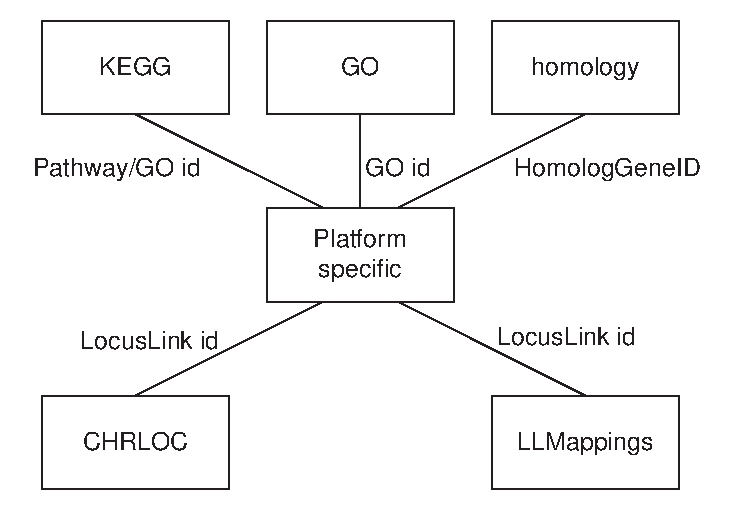
\includegraphics[width=\textwidth, angle=0]{DPChart}
%    \end{center}
%    \caption{{\small \label{fig:DPChart}A diagram showing the overall
%        structure and inter-relationship of Bioconductor annotation
%        data packages. Boxes show a single or group of data
%        packages. Lines between two boxes indicate connections through
%        the key denoted by the text beside each line.}}
% \end{figure*}

Each annotation library, when installed, contains a sqlite database contained
within the \texttt{extdata} along with a \texttt{man} subdirectory filled with
documentation about the data. The data can be accessed using the standard
methods that would work for the classic environment objects (hash table with
key-value pairs) and act as if they were simple associations of annotation
values to a set of keys. For each of these emulated environment objects (which
we will refer to as mappings), there is a corresponding help file in the
\texttt{man} directory with detail descriptions of the data file and usage.
In addition to the traditional access to these data, these databases can also
be accessed directly by using DBI interfaces which allow for powerful new
combinations of these data.

Each platform specific library creates a series of these mapping objects
named by following the convention of package name plus mapping
name. The package name is in lower case letters and the mapping
names are in capital letters. When a given mapping maps platform
specific keys to annotation data, only the name of the annotation data
is used for the name of the mapping. Otherwise, the mapping
names have a pattern of key name and value name joined by a "2" in
between. For example, \Robject{hgu95av2ENTREZID} maps probe ids on 
an Affymetrix human genome U95Av2 chip to EntrezGene IDs while \Robject{hgu95av2GO2PROBE} 
maps Gene Ontology IDs to probe IDs. Names of the mappings available in a
platform specific data package are not listed here to save space but
are easily accessible as shown later in the section for usage.


Genome level annotation libraries are named in the form of org.Xx.yy.db where
Xx represents an abbreviation of the genus and species. Each of the organism
wide genome anotation packages is based upon some type of widely used gene
based identifier (such as an Entrez Gene id) that is mapped onto all the other
features in the package.  The yy part of the name corresponds to this
designation, where eg means a package is an entrez gene package and sgd is a
package based on the sgd database etc.  In many cases the org packages will
contain more different kinds of information that the platform based ones,
since not all types of information are as widely sought after.


The \Rpackage{KEGG.db} library contains mappings between ids such as Entrez
Gene IDs and \Rpackage{GO} to \Rpackage{KEGG} pathway ids and thus also to
pathway names.  The \Rpackage{GO.db} library maintain the directed acyclic
graph structure of the original data from Gene Ontology Consortium by
providing mappings of GO ids to their direct parents or children for each of
the three categories (molecular function, cellular component, and biological
process). Mappings between Entrez Gene and \Rpackage{GO} ids are also
available to complement the the GO.db package. These mappings are found within
the organism wide packages mentioned above. These mappings are provided with
evidence code that specifies the type of evidence that supports the annotation
of a gene to a particular \Rpackage{GO} term.

\section*{Usage}

All the annotation libraries can be obtained from the Bioconductor web
site (\url{http://www.bioconductor.org}). To illustrate their usages,
we use the library for Affymetrix HG\_U95Av2 chip (\Rpackage{hgu95av2.db}) as
an example for platform specific data packages and the \Rpackage{GO.db} library for
non-platform specific data packages. We assume that R
(\url{www.r-project.org}) and Bioconductor's Biobase and annotation
libraries have already been installed.

\subsection*{Package installation}

Download libraries \Rpackage{hgu95av2.db} and \Rpackage{GO.db} with 
BiocManager::install(). If the \Rpackage{reposTools} library has already been
installed/loaded, typing \Rfunction{install.packages2(library name)} installs
the library for both Unix and Windows.

Typing library(library name) in an R session will load the library
into R. For example,

\begin{Schunk}
\begin{Sinput}
> library("annotate")